\documentclass{beamer}
% Example from https://www.overleaf.com/learn/latex/Beamer
% 
% 30.06.2021, nitr
% \usepackage{graphicx}
\usetheme{Madrid} % ganz angenehmes Theme

\usepackage[backend=biber]{biblatex} %biblatex mit biber laden
% \usepackage{biblatex}
\bibliography{Lit_smc.bib}

% Removes icon in bibliography
% \setbeamertemplate{bibliography item}{}


%Information to be included in the title page:
\title[Sliding Mode Control] %optional
{A short Introduction to Sliding Mode Control}

\subtitle{Robust Control for Nonlinear Systems}

\author[Rainer Nitsche] % (optional, for multiple authors)
{Dr.~Rainer~Nitsche\inst{1}} % \and J.~Doe\inst{2}}

\institute[Festo SE \& Co. KG] % (optional)
{
  \inst{1}%
  Dept. Robotics\\
 System Design Group
  % \and
  % \inst{2}%
  % Faculty of Chemistry\\
  % Very Famous University
}

\date[ \today] % (optional)
{Control Methods in Robotics, August 2021}

% \logo{\includegraphics[height=1cm]{overleaf-logo}}
\logo{
\includegraphics[height=2mmm]{FESTO_RGB_080}}
\begin{document}

\frame{\titlepage}

\begin{frame}
\frametitle{Sample frame title}
This is some text in the first frame. This is some text in the first frame. This is some text in the first frame.
\end{frame}

%<<FF>> ***********************************************************************
\begin{frame}
\frametitle{Some Remarks on SMC}
This is a text in second frame. 
For the sake of showing an example.

\begin{itemize}
 \item<1-> Text visible on slide 1
 \item<2-> Text visible on slide 2
 \item<3> Text visible on slide 3
 \item<4-> Text visible on slide 4
\end{itemize}
\end{frame}


% <<FF>> ***********************************************************************
% https://www.overleaf.com/learn/latex/Beamer_Presentations:_A_Tutorial_for_Beginners_(Part_2)%E2%80%94Lists,_Columns,_Pictures,_Descriptions_and_Tables#The_Description_Environment
\begin{frame}
  \frametitle{A motivating Example for SMC}

 \begin{columns}
   \column{0.5\textwidth}
   Sliding mode of the system:

   \begin{equation}
   \ddot x = \sin(3 t) + u 
   \end{equation}
     \column{0.5\textwidth}
   \centering
    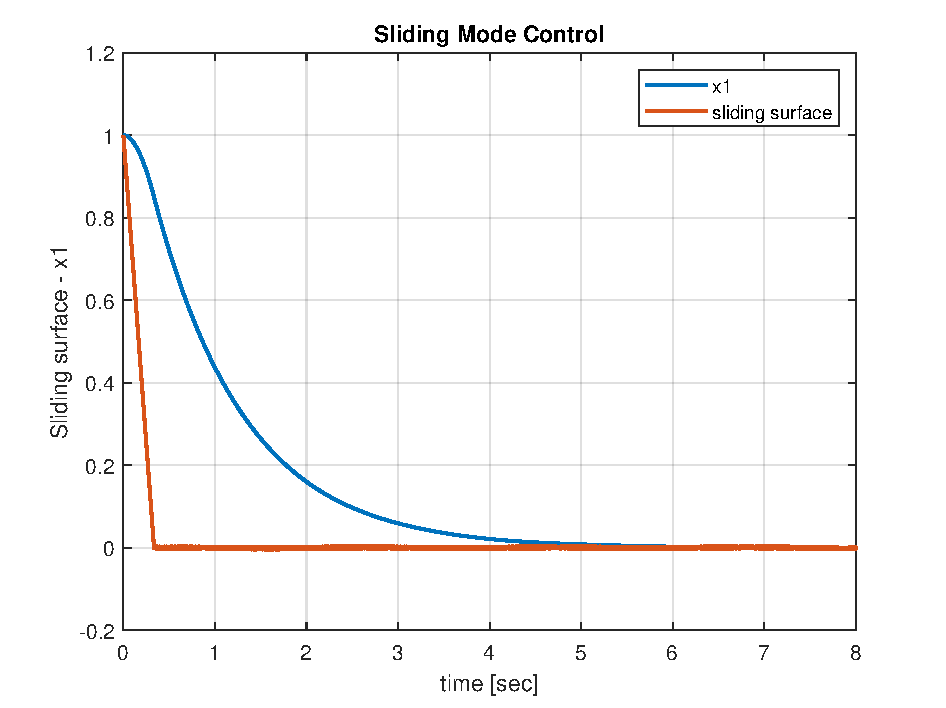
\includegraphics[height=4cm]{./pictures/SMCutkinRoadmap.pdf}
\end{columns}
 \end{frame}
%%% Local Variables:
%%% mode: latex
%%% TeX-master: "SMC4Students"
%%% End:



% <<FF>> ***************************************************
\begin{frame}
\frametitle{References}
% This prints the bibliography on the slide
\printbibliography
\end{frame}


\end{document}